%%%%%%%%%%%%%%%%%%%%%%%%%%%%%%%%%%%%%%%%%
% Short Sectioned Assignment
% LaTeX Template
% Version 1.0 (5/5/12)
%
% This template has been downloaded from:
% http://www.LaTeXTemplates.com
%
% Original author:
% Frits Wenneker (http://www.howtotex.com)
%
% License:
% CC BY-NC-SA 3.0 (http://creativecommons.org/licenses/by-nc-sa/3.0/)
%
%%%%%%%%%%%%%%%%%%%%%%%%%%%%%%%%%%%%%%%%%

%----------------------------------------------------------------------------------------
%       PACKAGES AND OTHER DOCUMENT CONFIGURATIONS
%----------------------------------------------------------------------------------------

\documentclass[paper=a4, fontsize=11pt]{scrartcl} % A4 paper and 11pt font size

\usepackage[T1]{fontenc} % Use 8-bit encoding that has 256 glyphs
\usepackage{fourier} % Use the Adobe Utopia font for the document - comment this line to return to the LaTeX default
\usepackage[english]{babel} % English language/hyphenation
\usepackage{amsmath,amsfonts,amsthm} % Math packages

\usepackage{lipsum} % Used for inserting dummy 'Lorem ipsum' text into the template

\usepackage{sectsty} % Allows customizing section commands
\allsectionsfont{\centering \normalfont\scshape} % Make all sections centered, the default font and small caps

\usepackage{fancyhdr} % Custom headers and footers
\pagestyle{fancyplain} % Makes all pages in the document conform to the custom headers and footers
\fancyhead{} % No page header - if you want one, create it in the same way as the footers below
\fancyfoot[L]{} % Empty left footer
\fancyfoot[C]{} % Empty center footer
\fancyfoot[R]{\thepage} % Page numbering for right footer
\renewcommand{\headrulewidth}{0pt} % Remove header underlines
\renewcommand{\footrulewidth}{0pt} % Remove footer underlines
\setlength{\headheight}{13.6pt} % Customize the height of the header

\numberwithin{equation}{section} % Number equations within sections (i.e. 1.1, 1.2, 2.1, 2.2 instead of 1, 2, 3, 4)
\numberwithin{figure}{section} % Number figures within sections (i.e. 1.1, 1.2, 2.1, 2.2 instead of 1, 2, 3, 4)
\numberwithin{table}{section} % Number tables within sections (i.e. 1.1, 1.2, 2.1, 2.2 instead of 1, 2, 3, 4)

\setlength\parindent{0pt} % Removes all indentation from paragraphs - comment this line for an assignment with lots of text

\usepackage{graphicx}
\graphicspath{ {./img/} }
\usepackage{float}

%----------------------------------------------------------------------------------------
%       TITLE SECTION
%----------------------------------------------------------------------------------------

\newcommand{\horrule}[1]{\rule{\linewidth}{#1}} % Create horizontal rule command with 1 argument of height

\title{
\normalfont \normalsize
\textsc{Department of Computer Science, University of Helsinki} \\ [25pt] % Your university, school and/or department name(s)
\horrule{0.5pt} \\[0.4cm] % Thin top horizontal rule
\huge Exercise3: Denoising and compression by PCA and FA \\ % The assignment title
\horrule{2pt} \\[0.5cm] % Thick bottom horizontal rule
}

\author{Han Xiao} % Your name

\date{\normalsize\today} % Today's date or a custom date

\begin{document}

\maketitle % Print the title

%----------------------------------------------------------------------------------------
%       PROBLEM 1
%----------------------------------------------------------------------------------------

\section{Question 1}

\begin{table}[H]
\caption{Left: orignal first 100 digits\newline Right: preprocessed first 100 digits}
\centering
\begin{tabular}{cc}
  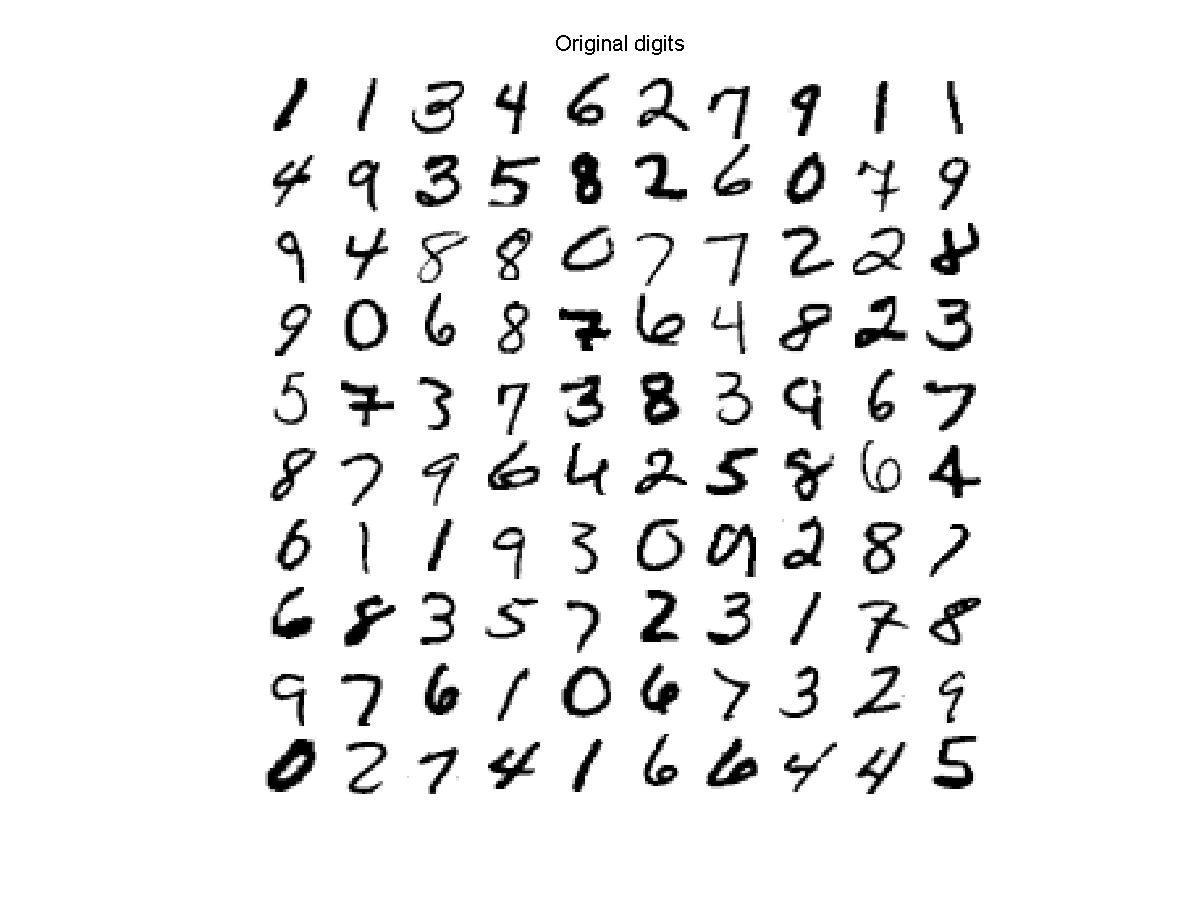
\includegraphics[scale=.4]{original_digits} &
  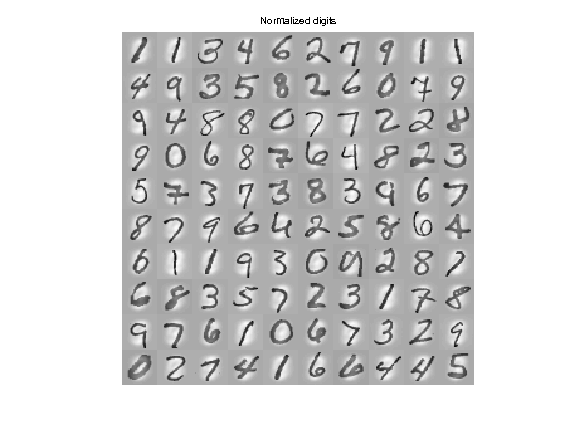
\includegraphics[scale=.4]{normalized_digits}
\end {tabular}
\end {table}



%------------------------------------------------


%----------------------------------------------------------------------------------------
%       PROBLEM 2
%----------------------------------------------------------------------------------------

\section{Question 2}

The first 20 principal components expained 64.449582\% of the variance.

\begin{figure}[H]
  \centering
  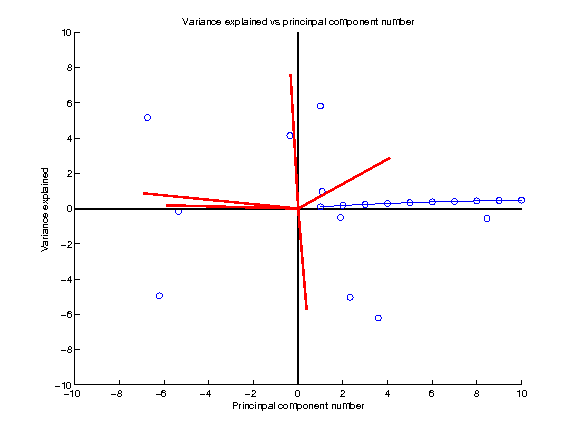
\includegraphics[scale=.7]{variance_explained}
  \caption{Proportion of variance explained vs number of principal component used}
\end{figure}


%----------------------------------------------------------------------------------------
%       PROBLEM 3
%----------------------------------------------------------------------------------------

\section {Question 3}

I randomly choose 10 digits from the dataset and project each of them to 1, 2, 4, 8, 16, 32, 64, 128 dimensional subspace and observed an increased level of restoration.

\begin{table}[H]
\caption{Randomly chosen digits before and after compression under PC number 1,2,4,8,16,32,64 and 128(left to right and updown)}
\centering
\begin{tabular}{cc}
	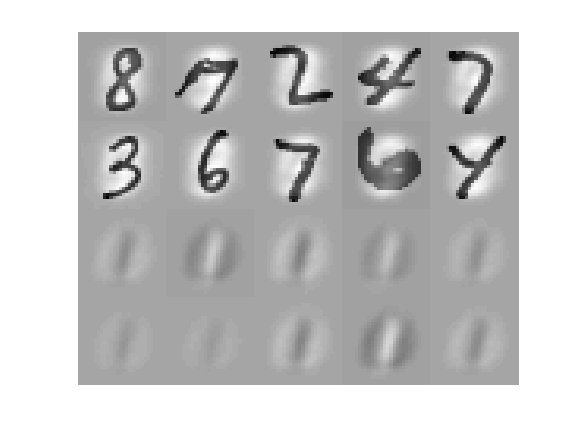
\includegraphics[scale=.3]{image_1}&
	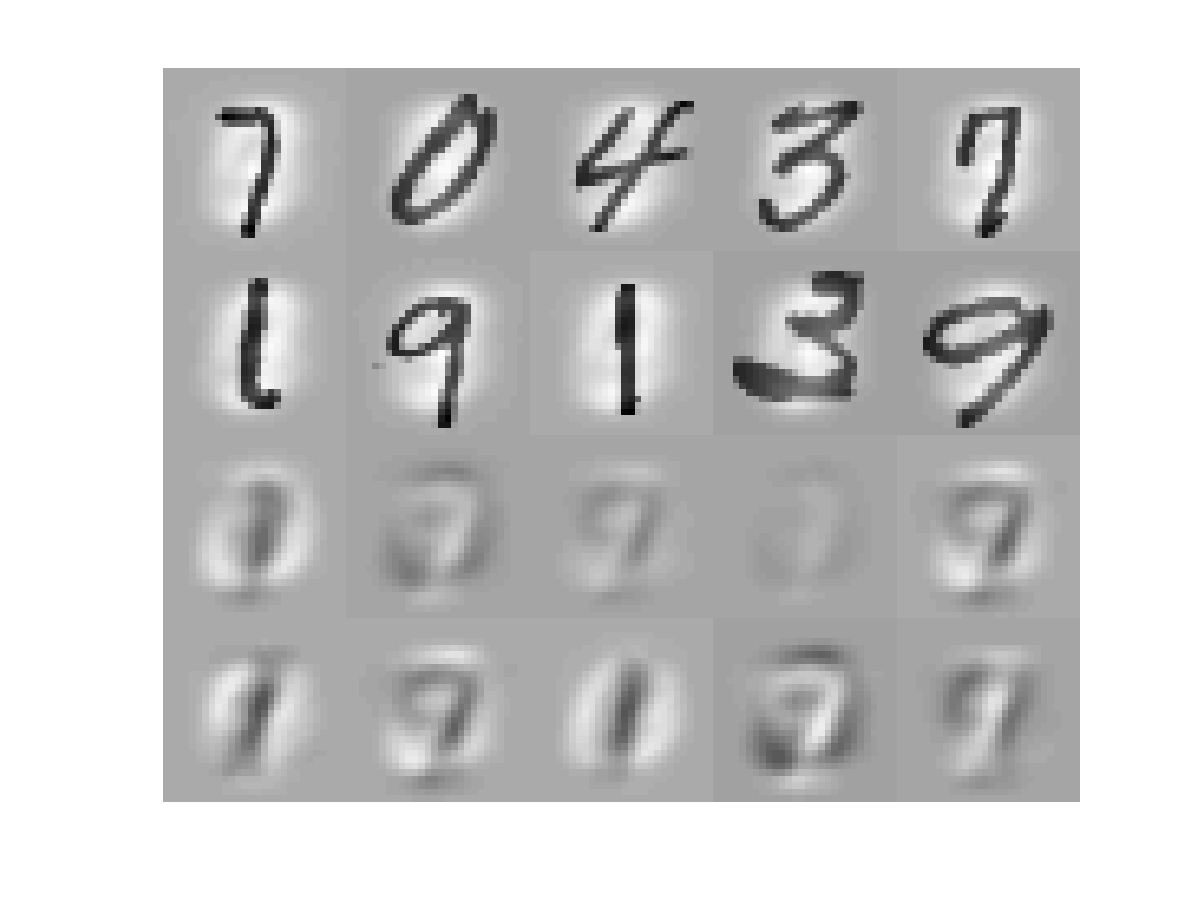
\includegraphics[scale=.3]{image_2}\\
	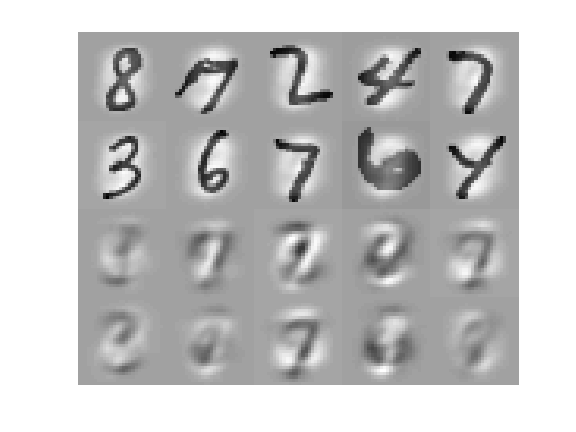
\includegraphics[scale=.3]{image_4}&
	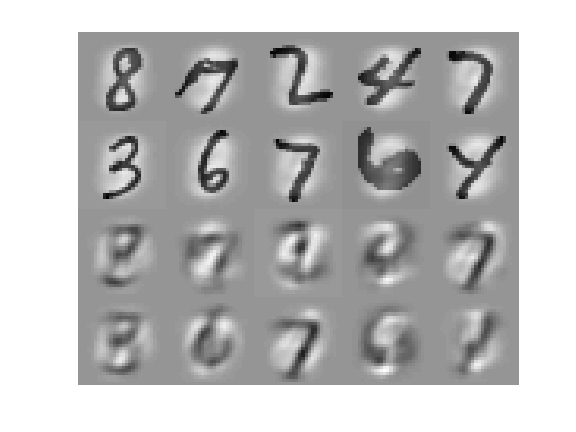
\includegraphics[scale=.3]{image_8}\\
	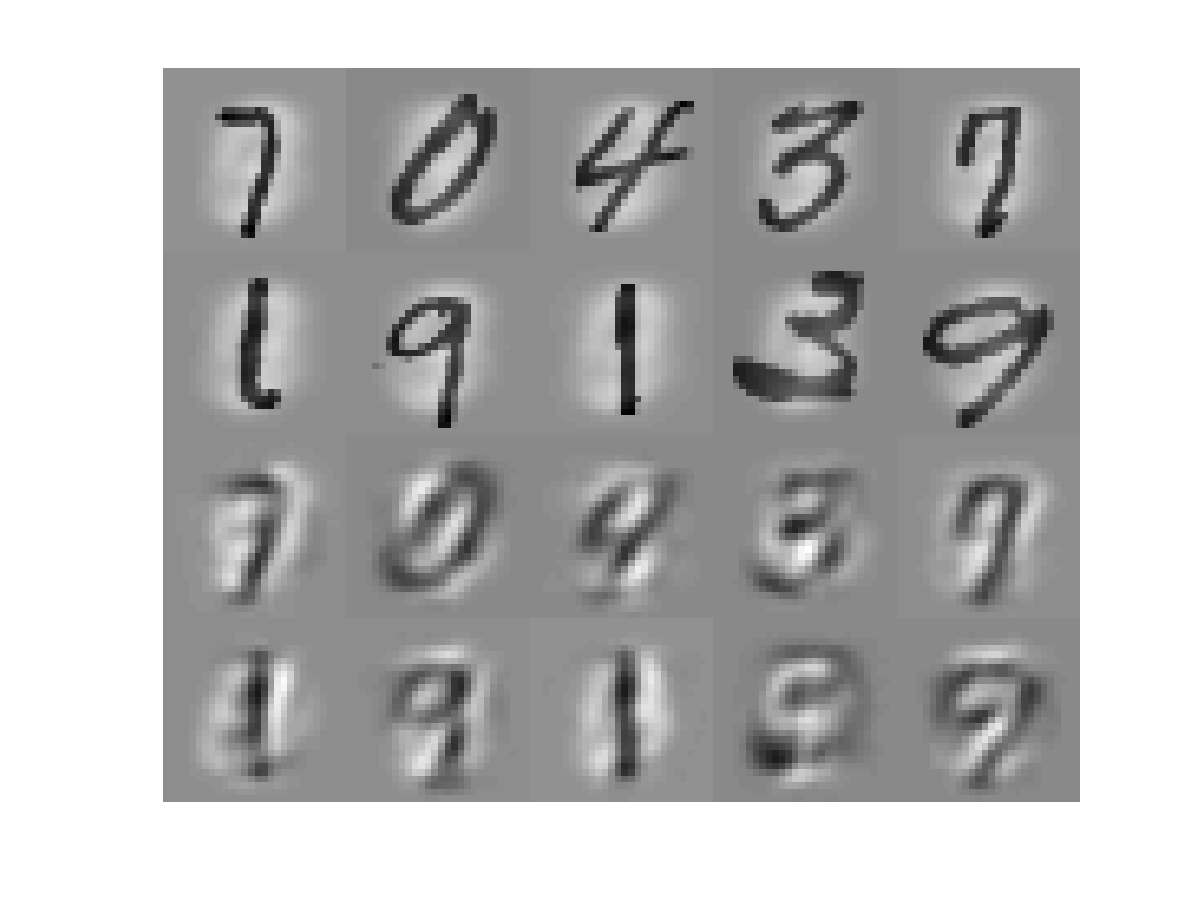
\includegraphics[scale=.3]{image_16}&
	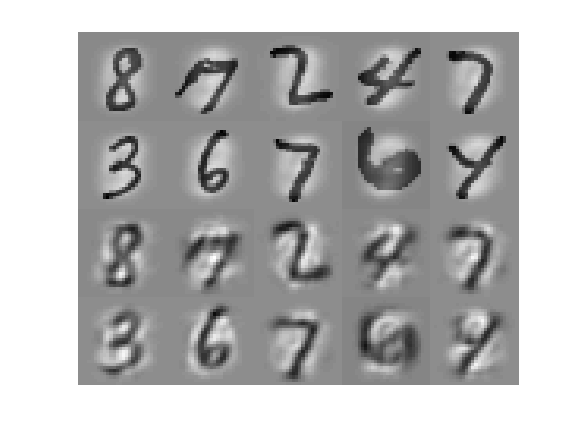
\includegraphics[scale=.3]{image_32}\\
	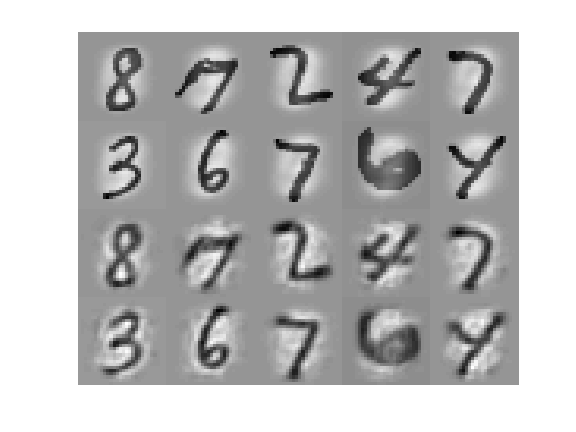
\includegraphics[scale=.3]{image_64}&
	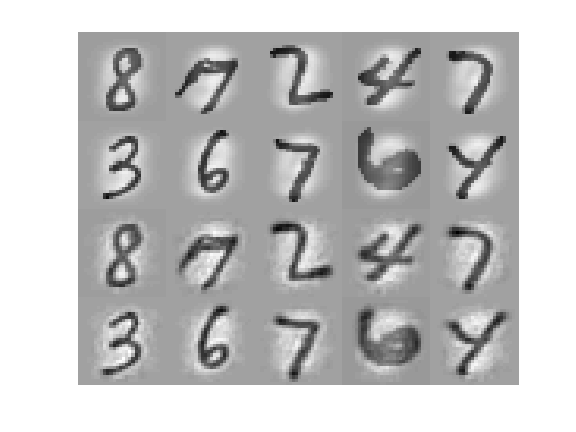
\includegraphics[scale=.3]{image_128}
\end{tabular}
\end{table}

\begin{table}[H]
\caption{Average reconstruction error for each dimension}
\centering
\begin{tabular}{c|cccccccc}
  Number of PC  &  1  &  2  &  4  &  8   \\  \hline
  Avg Error  &  89.858629\%  &  82.198814\%  &  71.321507\%  &  56.438138\%  \\ \hline
  Number of PC  & 16  &  32  &  64  &  128 \\  \hline
  Avg Error & 40.661514\%  &  25.329494\%  &  13.008691\%  &  5.313130\% 
\end{tabular}
\end{table}

%----------------------------------------------------------------------------------------
%       PROBLEM 4
%----------------------------------------------------------------------------------------

\section {Question 4}

I used the first 32 PC for denoising and the digits before and after denoising are as followed;

\begin{table}[H]
\caption{Denoising using 32 PC.\newline Left: original noisy digits \newline Right:denoised digits}
\centering
\begin{tabular}{cc}
    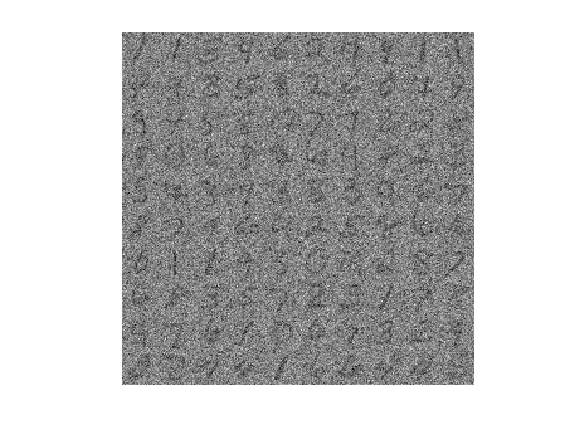
\includegraphics[scale=.4]{noisy_digits} &
    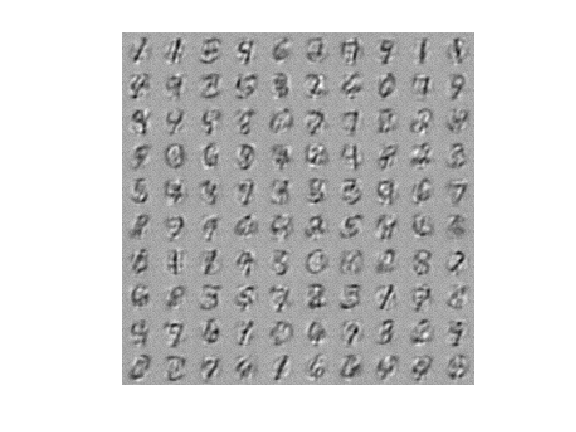
\includegraphics[scale=.4]{denoised_digits}
\end {tabular}
\end {table}

\end{document}
